\documentclass[a4paper,12pt,oneside,onecolumn,final,openright]{book}%Configuración de la clase... Cambiar draft-->final cuando esté terminado.
\usepackage[utf8]{inputenc}
\usepackage[a4paper,margin=0.2\textwidth]{geometry}%Márgenes
\usepackage[spanish]{babel}

\usepackage{amsmath,amsfonts,amssymb,mathtools}
\usepackage{bm}
\usepackage{tabto}

\usepackage{graphicx,float}
\usepackage[justification=centering]{caption}
\usepackage{subcaption}
\graphicspath{ {Images} }
\usepackage[pdftex]{hyperref}
\hypersetup{colorlinks=true,linkcolor=black,citecolor=black}
\addto\captionsspanish{
\renewcommand*\contentsname{Índice de contenidos}
\renewcommand*{\listfigurename}{Índice de figuras}
\renewcommand*{\listtablename}{Índice de símbolos}
}


\graphicspath{{Images}}




%%%%%%%%%%%%%%%%%%%%%%%%%%%%%%%%%%%%%%%%%%%%%%%%%%%%%%%%%%%%%%%%%%%%%%%
%% Carátula 
%%%%%%%%%%%%%%%%%%%%%%%%%%%%%%%%%%%%%%%%%%%%%%%%%%%%%%%%%%%%%%%%%%%%%%%
%\renewcommand{\maketitle}[0]{%
%  \thispagestyle{empty}
%    \vspace{-1cm}
%    \begin{center}
%      \begin{minipage}[t]{0.125\linewidth}
%        
\includegraphics[width=0.2cm]{logos/logo_univ.png}
%      \end{minipage}      
%      \hfill
%      \begin{minipage}[t]{0.73\linewidth}
%        \begin{center}%
%
%          \vspace{-1.6cm}
%          \textsc{\small Universidad Nacional de La Plata}\\
%          \textsc{\small Facultad de Ingeniería}
%          
%        \end{center}
%      \end{minipage}      
%      \hfill
%      \begin{minipage}[t]{0.125\linewidth}
%        
\includegraphics[width=0.2cm]{logos/logo_fiunlp.png}
%      \end{minipage}\\
%    \end{center}
%    \vspace{1cm}
%    \begin{center}
%      {\huge Estudio e Implementación del Protocolo RTCM para DGNSS en Tiempo Real}
%    \end{center}
%    \vspace{1cm}
%    \begin{center}
%      \begin{minipage}[t]{0.9\linewidth}
%        \begin{center}
%          \textsc{Tesina de grado presentada a la Facultad de Ingeniería de
%            la Universidad Nacional de La Plata
%            por}\\\vspace{0.5cm}{\large
%            Juan Fermín Llorente}\\\vspace{0.5cm}\textsc{en cumplimiento parcial
%            de los requerimientos\\ para la obtención del título
%            de\\Ingeniero en Telecomunicaciones.}
%        \end{center}
%      \end{minipage}
%    \end{center}
%
%    \vspace{2}
%
%    \begin{center}
%      \textsc{Directores}
%      \begin{minipage}[t]{0.9\linewidth}
%
%        Ing. Javier A. Smidt %
%        \dotfill{} %
%        UIDET SENyT, FI-UNLP %
%        
%        Ing. Ernesto M. López %
%        \dotfill{} %
%        UIDET SENyT, FI-UNLP %
%
%      \end{minipage}
%
%      \vspace{1cm}
%
%      \textsc{Tribunal}\\
%      \begin{minipage}[t]{0.9\linewidth}
%
%        Quien me vigile %
%        \dotfill{} %
%        de donde %      
%        \end{minipage}
%
%    \begin{minipage}[t]{0.9\linewidth}
%        \vspace{.5cm}
%        \centering
%        
\includegraphics[width=0.5\textwidth]{logos/senyt.png}\\
%        UIDET Sistemas Electrónicos de Navegación y Telecomunicaciones (SENyT)
%    \end{minipage}
%    
%    \vspace{3}
%    \vfill 
%
%    \begin{minipage}[t]{0.9\linewidth}
%    \centering
%        La Plata\\
%        10 de Diciembre, 2022
%    \end{minipage}
%    \end{center}
%
%}

\title{Tesina de grado - Ingeniería en Telecomunicaciones}
\author{Juan Fermín Llorente\\Directores\\jurados\\foto unlp\\foto senyt}
\date{Diciembre, 2022}

\begin{document}
\maketitle

% \frontmatter
\chapter*{Agradecimientos}
\addcontentsline{toc}{chapter}{Agradecimientos}
\newpage
\chapter*{Resumen/Abstract}
\addcontentsline{toc}{chapter}{Resumen/Abstract}
\newpage
\addcontentsline{toc}{chapter}{Índice de símbolos}
\chapter*{Índice de símbolos}
\newpage
\addcontentsline{toc}{chapter}{Índice de contenidos}
\tableofcontents
\newpage
\addcontentsline{toc}{chapter}{Índice de figuras}
\listoffigures


% \mainmatter
\chapter{Sistemas globales de navegación por satélite}
	Este capítulo introduce los primeros conceptos para el posicionamiento basado en sistemas de navegación por satélite. Incluye una breve descripción del sistema de posicionamiento global (GPS por sus siglas en inglés) junto con sus señales y las mediciones que pueden obtenerse mediante las mismas. Se hace hincapié en las características de estas señales, además de analizar las fuentes de error que hay presentes en las mismas.
	
\section{Introducción}
	Los sistemas GNSS (\textit{Global Navigation Satellite System} en inglés) se basan en el concepto de mediciones de rango mediante el retardo de propagación de las señales transmitidas por constelaciones de satélites. El tiempo de arribo (TOA por sus siglas en inglés) determina el instante en el que se recibió la señal, conociendo el instante en el que la misma fue transmitida se puede determinar el tiempo de viaje de la misma. Haciendo uso de la velocidad de propagación de la señal es posible obtener el rango en el que se encuentra el equipo transmisor. Introduciendo múltiples mediciones de rango con satélites transmitiendo en distintas ubicaciones se puede acotar la ubicación del receptor. La solución puntual queda determinada por el punto de intersección de las esferas formadas por el rango que se midió a cada uno de los satélites involucrados, siempre y cuando se tomen suficientes mediciones para poder resolver la posición de manera unívoca. 
	
	Habiendo introducido el concepto de medición de rango mediante TOA, es necesario analizar la sincronización entre las distintas partes que conforman el sistema. Si se busca resolver la posición mediante este concepto, las señales recibidas de los distintos satélites deben haber sido transmitidas en el mismo instante de tiempo. El instante de tiempo de toma de las observaciones tiene el nombre de época en este contexto. Es evidente que para conseguir esto los relojes de referencia de los satélites y del usuario (llamado receptor anteriormente) deben tener muy alta precisión y sincronización entre ellos. La precisión no es un inconveniente ya que los satélites GPS utilizan relojes atómicos que logran una estabilidad destacable (refe?). En cambio, la sincronización del usuario al tiempo del sistema GPS (al cual deberían estar sincronizados todos los satélites de la constelación), es un tanto más compleja y por ello se analizarán los errores que introducen las fallas en la sincronización.
	
	Existen distintos sistemas GNSS, tales como \textit{GPS}, \textit{Galileo}, \textit{Glonass} o \textit{BeiDou}, cada uno con su respectiva constelación de satélites MEO (\textit{Medium Earth Orbit} u Órbita Circular Intermedia). Si bien el foco de este trabajo está puesto en el mencionado primero, el sistema GPS, se desarrollan los conceptos de este capítulo de forma general para todos los sistemas. Todos los satélites de las distintas constelaciones comparten el canal de transmisión, esto es posible debido al uso de técnicas de acceso múltiple. En particular, el sistema GPS cuenta con 32 satélites operativos actualmente y como la frecuencia de operación es compartida por todos los satélites, el mismo utiliza acceso múltiple por división de código (CDMA por sus siglas en inglés). En cambio, el sistema \textit{Glonass} cuenta con 24 satélites operativos y cada uno transmite dentro de la misma banda de frecuencias multiplexando los canales por frecuencia dentro de esta banda. Esta técnica es conocida como acceso múltiple por división de frecuencia (FDMA por sus siglas en inglés).
	
\section{Características de la señal}\label{sec:senial}
	Las señales transmitidas se encuentran dentro del espectro de las radiofrecuencias. Existen distintos tipos de señales, según se fueron modernizando los sistemas, y en particular los satélites, se han ido sumando nuevas señales. Las características principales que componen a una señal de GPS son la frecuencia de portadora dentro de la banda \textit{L}, el código que hace posible el acceso múltiple y por último el mensaje de navegación.
	
	En cuanto a la frecuencia de portadora de la señal, para aplicaciones civiles se puede diferenciar la frecuencia primaria $L_1$ y frecuencia secundaria $L_2$. Ambas son múltiplos de una frecuencia fundamental $f_0=10.23$\,MHz. La señal en $L_1$ tiene una frecuencia de portadora igual a $154\cdot f_0 = 1.5754$\,GHz y la señal en $L_2$ igual a $120\cdot f_0 = 1.2276$\,GHz. Estas dos señales son las consideradas \textit{legacy} ya que fueron heredadas de los primeros bloques de satélites GPS que se hicieron operativos. También existe la señal en $L_5$, una señal mas moderna, pero que no es utilizada a lo largo de este trabajo por lo que solo se la menciona.
	
	Las señales son expandidas en el espectro mediante una secuencia de ruido pseudoaleatoria (\textit{PRN} por sus siglas en inglés), esta secuencia es el código que ya fue mencionado. Las técnicas de espectro expandido de secuencia directa (DSSS por sus siglas en inglés) utilizadas, distribuyen la energía de la señal de cada satélite en todo el ancho de banda disponible. De esta manera es posible mitigar efectos adversos naturales del canal como lo son el ruido o interferencias, además de presentar la ventaja de permitir el acceso múltiple entre usuarios estas técnicas presentan robustez frente a interferencias intencionadas. Esta última característica generaba gran interés al momento de creación del sistema GPS con fines militares. Se logra expandir la señal de manera tal que la misma queda oculta por el piso de ruido presente en el canal. El receptor, que conoce el código con el cual se hizo la expansión, logra recuperar la señal pudiendo incluso considerar a las señales del resto de los satélites como interferencias. 
	
	Los mensajes de navegación en GPS se transmiten con una tasa de 50\,bps, como la modulación es BPSK esto resulta en un ancho de banda de 50 Hz. Los símbolos transmitidos son de 20 ms de duración con conformación espectral idealmente dada por cajones. La información transportada por el mensaje de navegación es la que hace posible computar la posición de cada satélite y tiempo de transmisión de las señales. En los mismos se transmite, entre otras cosas, el mensaje de telemetría, al cual solo tienen acceso los usuarios autorizados, términos de corrección de reloj para desafectar errores en la medición y como componente principal, se transmiten las efemérides. Las efemérides contienen la información del tiempo del satélite (referenciado al tiempo GPS), parámetros keplerianos de las órbitas osculantes de los satélites.
	
	En términos generales, la polaridad de cada símbolo rectangular estará dada por el bit de información de navegación a transmitir. Luego se expande esta señal mediante el producto de la amplitud de cada símbolo con el código, la modulación por desplazamiento de fase de la señal resultante estará dominada por las transiciones del código. Un ejemplo de un código PRN se puede observar en la Fig. \ref{fig:PRN}, donde cada transición del código es denominado \textit{chip}. Es evidente que la tasa resultante de la señal BPSK multiplicada por el código es mucho mayor que la de la señal original, ya que en cada transición de símbolo tiene múltiples transiciones de \textit{chip}. La señal de espectro expandido tiene una tasa igual a la tasa de \textit{chip} $R_c$ tal que $R_c \gg R_b$, resultando en una expansión en el espectro.
\begin{figure}%Se puede agregar un indicador de chip en la imagen.
    \centering
    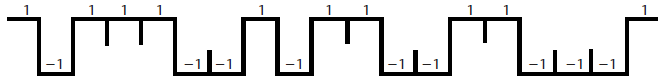
\includegraphics[width=0.8\textwidth]{GNSS/codigoPRN.png}
    \caption{Ejemplo de código PRN.}
    \label{fig:PRN}
\end{figure}

	Este mecanismo implica que el receptor conozca con exactitud el código utilizado en la expansión para poder multiplicar nuevamente a la señal por el mismo, considerando sincronización perfecta, y así recuperar la señal original. Este proceso se puede interpretar como la compresión de la señal expandida al momento de la transmisión, y en recepción es donde se recupera solo la señal de interés.
	
	Como ya fue mencionado, el sistema utiliza CDMA para multiplexar las señales de los distintos satélites. Cada satélite tiene una secuencia PRN que debe cumplir con las características de presentar autocorrelación muy similar a la de un proceso de ruido blanco, para su correcta recuperación en el receptor cuando hay sincronización. Y además debe tener muy baja intercorrelación con los códigos del resto de los satélites. Esta última condición es necesario extenderla para que cada PRN tenga baja intercorrelación con todos los posibles desplazamientos de los restantes códigos del sistema. Esto se debe a las variaciones de TOA de las diferentes señales y por el mecanismo de medición de tiempo de viaje de la señal que se detallará posteriormente. Las PRN que presentan estas características son las secuencias \textit{Gold} [cita a Proakis] y son las utilizadas en este sistema. Si los distintos códigos fueron diseñados (o elegidos) correctamente, las interferencias del resto de las señales no deseadas pueden ser consideradas como ruido aditivo a la señal de interés.
	
	Ya se introdujo el mecanismo de multiplexado de las señales de cada satélite y se detallaron algunos aspectos de las señales GPS. Las señales civiles mencionadas pueden estar expandidas por distintos códigos, que en conjunto con la frecuencia de portadora son los dos parametros que le dan nombre a las señales. Los códigos 
\begin{itemize}
	\item Código C/A: Es el código transmitido en la señal $L_1$, de la familia de códigos de largo 1023. Tiene una tasa de 1.023 Mchips/s por lo tanto tiene un periodo de \textit{chip} igual a 1 ms.
	\item Código P: Este código se repite una sola vez por semana, al comienzo de la semana GPS (dentro del sistema de tiempo GPS), por eso se lo menciona como código largo. Tiene un largo de $6,187104\cdot 10^{12}$ chips y se transmite a una tasa diez veces mayor que la del código C/A. El mismo es transmitido en la señal $L_1$ tanto como en la $L_2$.
\end{itemize}
	
\section{Formación de los observables}
	Para determinar la posición, el usuario debe medir los rangos a cada satélite y resolver su posición mediante la combinación de estas. Para lograr la solución de posición se utilizan distintas observaciones, 4 mediciones son necesarias para poder obtener la solución puntual. Pero también se puede utilizar información redundante para obtener una solución más confiable, pudiendo aplicar algún tipo de filtrado y obtener una mejor estimación. En la etapa del lazo de enganche de retardo (\textit{DLL} por sus siglas en inglés) se obtienen mediciones de pseudorango mediante la fase del código. Además, se pueden obtener mediciones de fase de portadora mucho más precisas pero a expensas de un nivel de ambigüedad en el rango que debe resolverse por otro camino.
	
	A través de estas mediciones es posible resolver el sistema de ecuaciones linealizadas para obtener la solución de posición. No nos centraremos en este proceso ya que el objetivo de este trabajo consiste en el análisis de las mediciones en diferencias para posicionamiento diferencial. 
	
\subsection{Medición de pseudorango}
	Esta medición de rango se basa en la medición del tiempo de viaje de la señal y es aquí donde se aprovechan las características de los códigos mencionados en la Sección \ref{sec:senial}. El receptor debe conocer el código (ya sea \textit{C/A} o \textit{P}) asociado al satélite que quiere recibir, esto se utiliza para generar una replica del mismo en el \textit{DLL} del receptor y de esta manera el mismo puede comparar el desfasaje que existe entre el código de la señal recibida con el generado internamente, obteniendo el tiempo de viaje de la señal. Ambos códigos se generan internamente en el receptor al inicio de la semana GPS y al medir el desfasaje entre la replica y el recibido se posiciona el TOA dentro de la semana GPS. En el caso del código \textit{C/A} hay una ambigüedad de 1 ms debido a su periodo, pero se obtiene el TOA en estas condiciones y haciendo uso del mensaje de navegación se logra una medida absoluta. En el caso del código \textit{P} se obtiene una ubicación dentro de la semana GPS y no existe tal ambigüedad. Para medir el desfasaje, el receptor desplaza en tiempo la replica hasta lograr correlación entre ambas señales, por esto es importante que la intercorrelación entre los códigos sea baja para todos los desplazamientos de los mismos. De esta manera se evitan falsas detecciones, solo consiguiendo correlación cuando hay sincronización con el código del satélite que se espera recibir.
	
	La ecuación de observación con medición de pseudorango es 
\begin{align}\label{ec:obs_pseudorango}
	p_{r,j}^s(t) = \rho_r^s(t) + \xi_{r,j}^s + c\left(d_{r,j}-d_j^s\right) + c\left(dt_r(t)-dt^s(t)+\delta t^{rel}(t)\right)& \\ 
	+ I_{r,j}^s(t) + T_r^s(t) +e_{r,j}^s(t)& \ . \nonumber
\end{align}

	Es necesario introducir los términos de la misma. La medición de pseudorango no es considerada rango por el hecho de que contiene los efectos de no sincronización entre los relojes del usuario y el satélite. 
\begin{itemize}
	\item $p_{r,j}^s(t)$: Pseudorango del usuario con el satélite obtenido con la ecuación de observación, siendo $j$ el identificador de las señales del mismo satélite.
	\item $\rho_r^s(t)$: Rango geométrico.
	\item $\xi_{r,j}^s$: Término de corrección debido a sesgos en los centros de fase de las antenas transmisora y receptora.
	\item $d_{r,j}$, $d_j^s$: Retardos instrumentales o de hardware en el receptor y en el satélite, respectivamente. Ambos medidos en segundos.
	\item $dt_r(t)$, $dt^s(t)$: Sesgos en el reloj del receptor y del satélite, respectivamente. Ambos medidos en segundos. 
	\item $\delta t^{rel}(t)$: Sesgo debido al efecto relativista. Medido en segundos. 
	\item $I_{r,j}^s(t)$, $T_r^s(t)$: Retardo ionosférico y troposférico, respectivamente. En unidades de metros.
	\item $e_{r,j}^s(t)$: Errores adicionales, tales como multicamino y por ruido térmico en el receptor.
\end{itemize}

\subsection{Medición de fase de portadora}%19.1.2 en el handbook.
	La misma se realiza en el lazo de enganche de fase (\textit{PLL} por sus siglas en inglés), midiendo los desfasajes de la portadora replica con la portadora recibida, la ambigüedad esta determinada por la longitud de onda de la portadora, que es muy baja. La misma estará en el rango de 19 cm a 25 cm, la longitud de onda más chica es la correspondiente a la señal $L_1$ y la mayor a $L_2$. En este enfoque no es posible salvar la ambigüedad haciendo uso del mensaje de navegación ya que se pierde la señal modulada en la portadora. Pero esta longitud de onda pequeña trae ventajas a la medición en términos de precisión, se logra una precisión mucho más alta que con la medición de pseudorango. La ecuación de observación con medición de fase de portadora es
\begin{align}\label{ec:obs_fasedep}
	\varphi _{r,j}^s(t) = \rho_r^s(t) + \zeta_{r,j}^s(t) + c\left( \delta_{r,j}^s - \delta_j^s \right) + c\left( dt_r(t) - dt^s(t) + \delta t^{rel}(t)\right) &\\ 
	- I_{r,j}^s(t) + T_r^s(t) + \lambda_j \left( \omega_r^s(t) + N_{r,j}^s \right) + \epsilon_{r,j}^s(t)& \ . \nonumber
\end{align}
\begin{itemize}
	\item $\varphi _{r,j}^s(t)$: Medición de fase de portadora entre el usuario y el satélite obtenido con la ecuación de observación, siendo $j$ el identificador de las señales del mismo satélite. En unidades de metros.
	\item $\rho_r^s(t)$, $dt_r(t)$, $dt^s(t)$, $\delta t^{rel}(t)$, $I_{r,j}^s(t)$, $T_r^s(t)$: Equivalentes a los términos en la Ecuación \ref{ec:obs_pseudorango}.
	\item $\zeta_{r,j}^s$: Término de corrección debido a sesgos en los centros de fase de las antenas transmisora y receptora.
	\item $\delta_{r,j}$, $\delta_j^s$: Retardos instrumentales o de hardware en el receptor y en el satélite, respectivamente. Ambos medidos en segundos.
	\item $\lambda_j$: Longitud de onda de la frecuencia j-ésima.
	\item $\omega_r^s(t)$: Corrección de wind-up de fase. Corresponde a cambios en la fase medida en caso de rotación de las antenas. En unidades de cantidades de longitudes de onda.
	\item $N_{r,j}^s$: El número entero de ciclos de la portadora presentes en la medición. Es un parámetro desconocido y está en unidades de cantidades de longitudes de onda.
	\item $\epsilon_{r,j}^s(t)$: Errores adicionales, tales como multicamino y por ruido térmico en el receptor.
\end{itemize}
Cabe destacar que los términos que representan los mismos fenómenos que en la Ecuación \ref{ec:obs_pseudorango} pero tienen distintos símbolos, es debido a que tienen distinta naturaleza. 

	Los términos desconocidos son obtenidos al resolver el sistema de ecuaciones linealizadas ya mencionado, sin embargo, se pueden observar múltiples épocas y de esta manera realizar una estimación de estos parámetros. No solo se estiman los términos correspondientes a los errores de rango, si no también se incluye la ambigüedad de fase de portadora. En principio, todos los términos desconocidos de la Ecuación \ref{ec:obs_fasedep} son estimados. 
\section{Errores}\label{sec:errores}
	Es de particular interés para este trabajo analizar la naturaleza de los términos de error que están involucrados en las Ecuaciones \ref{ec:obs_pseudorango} y \ref{ec:obs_fasedep}. Será de gran utilidad a la hora de trabajar con observaciones en diferencias. 
\subsection{Error en el reloj del satélite y usuario}
	El término que hace referencia a este fenómeno del lado del satélite es $dt^s(t)$. Es necesario aclarar que los satélites \textit{GPS} cuentan con relojes atómicos de elevada estabilidad, por lo que los errores son principalmente debido a sesgos entre el sistema de tiempo \textit{GPS} y el tiempo propio del satélite. El segmento de tierra se encarga de enviar las correcciones necesarias para corregir este error, haciendo que la diferencia entre el tiempo del satélite y la del sistema \textit{GPS} sea menor a 1 ms. 
	
	En cuanto al error del usuario, denotado $dt_r(t)$, es una medida de desincronización del reloj del usuario con el sistema \textit{GPS} (al cual deberían estar sincronizados los satélites. 
\subsection{Retardos instrumentales en satélite y usuario}
	Corresponden a sesgos en la etapa de procesamiento, ya sea analógico o digital. El término dependiente del satélite ($d_j^s$), es causado por diferencias de retardo en el camino analógico y digital de la unidad de generación de la señal y de la antena, que no son iguales para las distintas señales. Este término es asumido igual para todos los receptores recibiendo la misma señal. El correspondiente al receptor del usuario ($d_{r,j}$), es causado por diferencias de camino de la señal desde la antena al correlador. Son asumidos iguales para todas las señales del mismo tipo que son recibidas por el mismo usuario.
	
	 Cabe destacar que la parte principal de esta componente de sesgo no corresponde a la sección analógica del receptor, sino a la cadena de procesamiento digital de la señal (\textit{DSP} por sus siglas en inglés) [cita a Handbook 19.6.2]. De manera que son sesgos que se pueden eliminar mediante calibración del receptor.
	 
\subsection{Sesgo debido al efecto relativista}
	Este término aparece como $\delta t^{rel}(t)$ en la ecuación de observación. El reloj del satélite sufre desviaciones en frecuencia respecto a uno que se encuentra en tierra, debido al movimiento del satélite y los cambios en el potencial gravitatorio. Para compensar este efecto (atribuido a la relatividad especial y general) los relojes no trabajan exactamente a la frecuencia necesaria para generar las señales $L_1$ y $L_2$, sino que generan una frecuencia levemente menor. De esta manera, cualquier usuario en tierra recibe la señal compuesta con los efectos relativistas, y observa la frecuencia sin desviación. Sin embargo, esta corrección efectuada en el satélite, no corrige todo tipo de error ya que las órbitas de los satélites \textit{GPS} no son perfectamente circulares. Se agrega entonces una contribución al corrimiento en frecuencia debido a la excentricidad no nula de la órbita. Por otro lado, existe una contribución debido al efecto \textit{Shapiro}, un retardo en la señal debido al campo gravitacional de la tierra. 
	
	 Estas contribuciones son las que conforman el término ya mencionado en la ecuación de observación. 
	 
\subsection{Retardo ionosférico}
	Uno de los dos efectos atmosféricos presentes en la medición de las señales \textit{GPS} es el debido a la ionosfera. El hecho de que la ionosfera sea un medio dispersivo genera diferentes retardos a las distintas componentes de la señal, en particular la señal se atrasa frente a la fase de portadora, este efecto es conocido como divergencia ionosférica. Las variaciones en el índice de refracción que sufre la ionosfera se deben a cambios que existen en el contenido total de electrones (TEC por sus siglas en inglés), estos cambios se comportan con una dinámica lenta por lo que realizando mediciones en una suficiente cantidad de épocas puede proveer una buena estimación de la corrección a realizar. Por otro lado, se pueden realizar mediciones a doble frecuencia para aprovechar la dependencia del retardo con la misma, y así estimar la corrección. 
	
	Para los fines del posicionamiento diferencial en el que se centra este trabajo, es importante remarcar que el TEC de la ionosfera es dependiente de la zona, debido a cuestiones climáticas y de incidencia solar. Este aspecto será de gran utilidad a la hora de analizar combinación de múltiples mediciones entre receptores con distinta ubicación.
\subsection{Retardo troposférico}
	El retardo debido a la tropósfera está asociado a las irregularidades que existe en el indice de refracción de la misma, es un efecto que afecta a la señal en la última etapa del camino que recorre desde el satélite hasta el usuario, si el mismo se encuentra en tierra. No se observan variaciones a gran escala del índice de refracción, por lo que la troposfera es un medio no dispersivo en la banda de GPS (banda L). Se puede separar en dos componentes, la componente seca es predominante (se lleva un 90\% de la contribución total de este efecto) y tiene alto grado de predictibilidad. El otro 10\% es denominado la componente húmeda y no es tan sencillo de predecir. La separación se hace según la altura de la capa, siendo la componente seca la correspondiente a la parte inferior de la atmósfera (troposfera) y la componente húmeda la capa superior a la troposfera (estratosfera aunque en estas aplicaciones se consideran como un conjunto).

	Los dos términos de retardo atmosférico son altamente dependientes del ángulo de elevación que existe entre el usuario y el satélite interceptado. Esto es evidente debido a que la cantidad de atmósfera que atraviesa la señal es menor cerca del cenit y mayor para ángulos de elevación pequeños.
\subsection{Errores adicionales}
	Los errores adicionales pueden provenir de distintas fuentes o tener naturalezas completamente diferentes, pero de igual manera se juntan todas estas contribuciones en un término adicional. En principio este término contiene el ruido térmico del receptor y los errores debido al multicamino.
\section{Determinación de la posición} 
\chapter{GNSS diferencial}
 A fin de poder discutir la cancelación de estos términos al utilizar múltiples observaciones para construir mediciones en diferencias. Esto último nos dará el pie para desarrollar sobre los sistemas de posicionamiento diferencial, en los cuales se centra este trabajo.
\section{Múltiples mediciones combinadas}
	La acción de tomar múltiples mediciones y combinarlas para poder cancelar algunos de los términos, es de gran utilidad, y uno de los principales fundamentos para el posicionamiento diferencial en el que esta centrado este trabajo. Resulta de particular interés para poder proveer soluciones de posición más precisas, conocer los términos de error presentes en las ecuaciones de observación (Sección \ref{sec:errores}). Para esto se aprovecha la correlación espacial y temporal que existe entre algunos de estos fenómenos para las distintas mediciones, ya sea modificando la geometría del problema, u observando época a época. Las múltiples mediciones pueden hacer uso de señales de múltiples satélites con un receptor único o de una única señal recibida por múltiples receptores.
\subsection{Únicas diferencias}\label{sec:SD}
	Las observaciones combinadas de únicas diferencias entre receptores (BRSD por sus siglas en inglés) consisten en la diferencia de observaciones de un único satélite, usando dos receptores distintos. También se puede realizar la diferencia de observaciones de dos señales (satélites) en el mismo receptor (BSSD por sus siglas en inglés), la cual se denomina únicas diferencias entre satélites. Cabe destacar que las diferencias no necesariamente son entre observaciones básicas simples, se podrían diferenciar observaciones combinadas. Aquí se analizaran diferencias simples, sin combinación, por lo que las únicas diferencias serán mencionadas también como simples diferencias sin hacer distinciones.
	La nomenclatura correspondiente a cada medición es $\nabla$ para simples diferencias entre satélites y $\Delta$ cuando es entre receptores. Además se agregan índices para poder identificar a los receptores y satélites. En el superíndice se indica al satélite (o par de satélites diferenciados) y en el subíndice se indica al receptor (o par de receptores diferenciados).

\subsubsection{Entre receptores}
	El pseudorango resultante de la BRSD es
\begin{align}\label{ec:BRSD_pr}
	\Delta p_{12}^k &= p_2^k - p_1^k = \rho_{12}^k +cd_{12}^k + \xi_{12}^k + c\left( dt_{12} + \delta t_{stc,12}^{rel,k} \right) + I_{12}^k(bl) + T_{12}^k(bl) + e_{12}^k \ .
\end{align}
	La fase de portadora que se forma es
\begin{align}\label{ec:BRSD_fdp}
	\Delta \varphi_{12}^k &= \varphi_2^k - \varphi_1^k = \rho_{12}^k + c\left( dt_{12} + \delta t_{stc,12}^{rel,k} \right) + c\delta_{12}^k + \zeta_{12}^k - I_{12}^k(bl) + T_{12}^k(bl) + \lambda \left( \omega_{12}^k + N_{12}^k \right) + \epsilon_{12}^k \ .
\end{align}
	Se puede observar como se cancelan los términos que son compartidos, tales como el retardo instrumental del satélite y el sesgo en el reloj del satélite. Se conserva el término de retardo de instrumental diferencial en el receptor, debido a que solo podría cancelarse en caso de que ambos receptores cuenten con etapas idénticas de correladores. Por otro lado, los términos correspondientes a los retardos atmosféricos pasan a ser dependientes de la linea de base entre ambos receptores. Esto se debe a la correlación espacial que tienen estos fenómenos, cuanto menor sea la linea de base se puede considerar que estos términos son eliminados debido a que la señal atraviesa fragmentos de la atmósfera con similares características.
	
	En la medición de fase de portadora en simples diferencias se agregan el término de corrección de \textit{wind-up} de fase y de ambigüedad entera de fase, ambos diferenciales.
	
\subsubsection{Entre satélites}
	El pseudorango para el caso BSSD resulta
\begin{align}\label{BSSD_pr}
	\Delta p_1^{k1} = p_1^1 - p_1^k = \rho_1^{k1} + c\left( dt^{k1} + \delta t^{rel,k1} \right) + cd_1^{k1} + \xi_1^{k1} + T_1^{k1} + I_1^{k1} + e_1^{k1} \ .
\end{align}
	Y para la fase de portadora 
\begin{align}\label{BSSD_fdp}
	\Delta \varphi_1^{k1} = p_1^1 - p_1^k = \rho_1^{k1} + c\left( dt^{k1} + \delta t^{rel,k1} \right) + c\delta_1^{k1} + \zeta_1^{k1} + T_1^{k1} - I_1^{k1} + \epsilon_1^{k1} &\\
	+ \lambda^1\left( \omega_1^1 + N_1^1 \right) - \lambda^k\left( \omega_1^k + N_1^k \right)& \ . \nonumber
\end{align}
	En este caso los términos que se cancelarán son los compartidos debido a que se utiliza un único receptor. En particular, el retardo de hardware diferencial correspondiente al receptor y el sesgo de reloj del receptor debido al efecto relativista son cancelados. Se mantiene el retardo diferencial de los satélites. Los efectos atmosféricos pueden estar correlacionados o no, según si los satélites adquiridos se encuentran en posiciones cercanas o no. Como esta situación no resulta común y en principio se puede adquirir cualquier par de satélites, se considera para el caso general que los retardos debido a los efectos atmosféricos se mantienen.
\subsection{Dobles diferencias}
	Las mediciones en dobles diferencias (DD de aquí en más) se construyen mediante la diferenciación de dos simples diferencias, se pueden diferenciar dos mediciones BRSD con dos satélites distintos o dos mediciones BSSD con dos receptores distintos. Es evidente que será necesario contar con disponibilidad de un par de receptores y un par de satélites en vista para ambos receptores. Este tipo de mediciones son de particular interés ya que logran cancelar otros términos que las mediciones de simples diferencias detalladas en la Sección \ref{sec:SD} no lograban. La notación adoptada para las mediciones de dobles diferencias es $\Delta \nabla p_{12}^{1k}$ en el caso de pseudorango y para fase de portadora resulta equivalente. 
	
	La medición en DD con dos mediciones BRSD para pseudorango resulta
\begin{equation}\label{ec:DD_pr}
	p_{12}^{k1} = p_{12}^1 - p_{12}^k = \rho_{12}^{k1} + \xi_{12}^{k1} + T_{12}^{k1}(bl) + I_{12}^{k1}(bl) + e_{12}^{k1} \ .
\end{equation}
	En el caso de fase de portadora se obtiene
\begin{align}\label{ec:DD_fdp}
	\varphi_{12}^{k1} = \rho_{12}^{k1} + \zeta_{12}^{k1} + T_{12}^{k1} - I_{12}^{k1}	+\lambda \left( \omega_{12}^{k1} + N_{12}^{k1}\right) + \epsilon_{12}^{k1} \ .
\end{align}
	En estas mediciones se logra cancelar los sesgos de reloj del receptor que no se habían cancelado en las Ecuaciones \ref{ec:BRSD_pr} y \ref{ec:BRSD_fdp}. Además el término diferencial de corrección relativista es eliminado ya que son iguales para todas las mediciones de BRSD sin importar qué satélite se tome. Los retardos instrumentales diferenciales entre los receptores se cancelan por utilizar el mismo par de receptores, en caso de estos receptores estén diseñados de manera correcta y se puede considerar que los retardos no difieren entre canales. Los términos de retardo atmosférico se mantendrán siempre y cuando no haya correlación entre las mediciones, es por esto que es explicita la dependencia de los mismo con la longitud de la linea de base, para lineas de base no muy grandes estos términos son tan pequeños que pueden ser despreciados.

\subsection{Triples diferencias}
	Además de la correlación espacial que tienen los fenómenos que todavía no se han cancelado completamente, los mismos cuentan con una correlación temporal que no se ha podido tener en cuenta todavía. Esto se debe a que las mediciones en SD y DD, todas son haciendo diferencias de observaciones en la misma época. Las mediciones en triples diferencias se realizan mediante dos DD pero en distintas épocas, esto permite sacar provecho de la dinámica lenta que tienen las efectos atmosféricos. La notación tomada para identificar estas mediciones es $\partial p_{12}^{k1}$.
	
	La medición en triples diferencias de pseudorango y fase de portadora resulta
\begin{align}
	\partial p_{12}^{k1} = p_{12}^{k1}(t_i) - p_{12}^{k1}(t_{i-1}) = \partial\rho_{12}^{k1} + \partial\xi_{12}^{k1} + \partial T_{12}^{k1}(\Delta t) + \partial I_{12}^{k1}(\Delta t) + \partial e_{12}^{k1} \ ,
\end{align}
\begin{align}
	\partial \varphi_{12}^{k1} = p_{12}^{k1}(t_i) - p_{12}^{k1}(t_{i-1}) = \partial\rho_{12}^{k1} + \partial\zeta_{12}^{k1} + \partial T_{12}^{k1}(\Delta t) - \partial I_{12}^{k1}(\Delta t) + \partial \epsilon_{12}^{k1} + \partial\omega_{12}^{k1}\ .
\end{align}
	Además de los términos que ya no estaban presentes en las DD y lo que se han reducido las contribuciones atmosféricas, según qué tan grande es la diferencia de épocas tomada $\Delta t = t_{i-1}-t_i$ en comparación con la dinámica del fenómeno, podremos despreciar aún más estos términos. Es evidente que si la correlación espacial presente en los términos no fue suficiente como para despreciarlos, con un correcto diseño en este enfoque se consigue despreciarlos definitivamente.
\subsection{Linea de base nula}
	Este enfoque para armar las observaciones puede ser utilizado ya sea con simples diferencias tanto como con dobles diferencias. Es un caso particular de las ya mencionadas donde se utiliza la misma antena para ambos receptores, se divide la señal y cada receptor hace sus mediciones. Esto consigue que la correlación espacial sea completa debido a que la linea de base nula implica que los receptores estén ubicados en el mismo punto, por lo que la señal recorre el mismo camino para ambos receptores, es decir, es afectada por los mismos fenómenos. 
	
	En el caso de SD, se mantiene el término de sesgo debido al reloj del receptor y retardo de hardware. En cambio, para DD se logra cancelar el término del reloj. En mediciones de pseudorango este término termina siendo el único presente además de los errores adicionales de carácter aleatorio (multicamino es cancelado en caso de trabajar con un solo satélite y los dos receptores con misma antena). Para las mediciones de fase de portadora se eliminará el factor de \textit{wind-up} ya que la antena receptora es la misma, aunque se mantiene la ambigüedad de fase entera.
\section{Resolución de ambigüedades en mediciones de fase de portadora}
\section{Ecuaciones de observación}
\section{Real Time Kinematics}
Necesario introducir conceptos como base y rover.
\section{Estándar RTCM}
Lo que recolecté del estándar.
\subsection{Formato del mensaje}
\subsection{Mensaje de la estación de referencia estacionaria}
\subsection{Mensajes de múltiples señales}
\subsubsection{Empaquetado del pseudorango y fase de portadora}
\chapter{Ensayos con base y rover estacionarios utilizando receptores comerciales}
Arquitectura de ambos receptores. Modos de funcionamiento por arriba. Ensayo con Rx u-blox.
% \section{Arquitectura del receptor}
\section{Placa de evaluación F9P u-blox}
\subsection{Software de evaluación u-center}
% \section{Ensayos con base y rover estacionarios}
\section{Desempeño y calidad de la solución en el ensayo}
\chapter{Implementación de la transmisión de correcciones RTCM en un sistema embebido} 

\section{Receptor Q Series propietario de SENyT}
Arquitectura de ambos receptores. Modos de funcionamiento por arriba. 
\subsection{Arquitectura del receptor}
\subsection{Modo de funcionamiento}
\subsection{Manejo de tiempos en el receptor}

\section{Generación de mediciones}
\subsection{Sincronización al tiempo GPS y corrección de las mediciones}

\section{Pila de comunicación asociada a la interfaz RTCM}
Empaquetado del mensaje.
\subsection{Capa de protocolo}
\subsection{Capa de transporte}

\chapter{Validación en tiempo real}
\section{Solución de posición utilizando correcciones diferenciales}
\section{Resolución de ambigüedades fijas}
\subsection{Embrace mediocrity and pray for BART}
\chapter{Validación mediante post procesamiento}
\chapter*{Conclusiones generales}
\addcontentsline{toc}{chapter}{Conclusiones generales}
\section*{Trabajo a futuro}
\addcontentsline{toc}{section}{Trabajo a futuro}
\chapter*{Referencias}
\addcontentsline{toc}{chapter}{Referencias}
\end{document}

%Desfazaje X - Desfasaje OK
%¿Abreviaciones que esten en ingles (GPS, TOA, PRN, etc) van en italicas?

